\documentclass[11pt,a4paper]{article}
\usepackage[utf8]{inputenc}
\usepackage[margin=1in]{geometry}
\usepackage{amsmath,amssymb}
\usepackage{graphicx}
\usepackage{booktabs}
\usepackage{hyperref}
\usepackage{microtype}
\usepackage{xcolor}

\hypersetup{
    colorlinks=true,
    linkcolor=blue,
    citecolor=blue,
    urlcolor=blue
}

\title{\textbf{Implementation and Consistency Analysis of Longitudinal Current Correlations $J_L(Q,t)$ and Spectral Density $C_L(Q,\omega)$}}
\author{Trajectory Analysis for LAMMPS Toolkit}
\date{\today}

\begin{document}

\maketitle

\begin{abstract}
This report summarizes the implementation, theoretical foundations, and numerical verification of the longitudinal current correlation function $J_L(Q,t)$ and its spectral density $C_L(Q,\omega)$ within the CUDA Fortran dynamics module of the \texttt{trj\_analysis} suite. We discuss the continuity equation linking density and current fluctuations, the physical interpretation of Brillouin acoustic peaks for extracting sound velocities, and the origin of discrepancies observed at large $Q$ between collective and self correlations.
\end{abstract}

\section{Theoretical Foundations}

In molecular dynamics analysis of simple liquids, collective microscopic dynamics are characterized by density fluctuations $\rho(\mathbf{Q},t) = \sum_{j=1}^N e^{i \mathbf{Q} \cdot \mathbf{r}_j(t)}$ and longitudinal current density fluctuations:
\begin{equation}
j_L(\mathbf{Q},t) = \sum_{j=1}^N \left[ \mathbf{v}_j(t) \cdot \hat{\mathbf{Q}} \right] e^{i \mathbf{Q} \cdot \mathbf{r}_j(t)}, \quad \text{where } \hat{\mathbf{Q}} = \frac{\mathbf{Q}}{|\mathbf{Q}|}.
\end{equation}

The intermediate scattering function $F(Q,t)$ and the longitudinal current correlation function $J_L(Q,t)$ are defined as:
\begin{align}
F(Q,t) &= \frac{1}{N} \left\langle \rho(\mathbf{Q},t) \rho(-\mathbf{Q},0) \right\rangle, \\
J_L(Q,t) &= \frac{1}{N} \left\langle j_L(\mathbf{Q},t) j_L(-\mathbf{Q},0) \right\rangle.
\end{align}

\subsection{Continuity Equation and Derivative Relation}
Particle conservation dictates the continuity equation in Fourier space:
\begin{equation}
\frac{\partial \rho(\mathbf{Q},t)}{\partial t} = i Q j_L(\mathbf{Q},t).
\end{equation}
Taking the second time derivative of $F(Q,t)$ yields:
\begin{equation}
\frac{\partial^2 F(Q,t)}{\partial t^2} = - Q^2 J_L(Q,t) \quad \implies \quad J_L(Q,t) = -\frac{1}{Q^2} \frac{\partial^2 F(Q,t)}{\partial t^2}.
\end{equation}

In the frequency domain, taking the Fourier transform $\mathcal{F}$ yields the dynamic structure factor $S(Q,\omega) = \mathcal{F}\{F(Q,t)\}$ and the longitudinal current spectrum $C_L(Q,\omega) = \mathcal{F}\{J_L(Q,t)\}$:
\begin{equation}
C_L(Q,\omega) = \frac{\omega^2}{Q^2} S(Q,\omega).
\end{equation}

\subsection{Initial Value Limits}
At $t = 0$, the self longitudinal current correlation $J_{L,s}(Q,0)$ satisfies the equipartition limit:
\begin{equation}
J_{L,s}(Q,0) = \left\langle v_{L,i}^2(0) \right\rangle = \frac{k_B T}{m},
\end{equation}
providing a direct check of kinetic temperature and velocity projection consistency.

\section{CUDA Fortran Implementation}

The GPU pipeline was expanded in \texttt{src/modules/dynamics.cuf}:
\begin{enumerate}
    \item \textbf{GPU Pass (\texttt{FqtnD})}: Evaluates $v_{L,i}(t) = \mathbf{v}_i(t) \cdot \hat{\mathbf{Q}}$ in parallel with phase factors $e^{i \mathbf{Q} \cdot \mathbf{r}_i}$, accumulating $F(Q,t)$ and $J_L(Q,t)$ concurrently without additional memory transfers.
    \item \textbf{1D FFTW Pipeline (\texttt{print\_rtcor})}: Performs 1D FFTs on $J_L(Q,t)$ and $J_{L,s}(Q,t)$ to compute $C_L(Q,\omega)$ and $C_{L,s}(Q,\omega)$.
    \item \textbf{File Suite}: Outputs time correlations to \texttt{jqt.dat}, spectral densities to \texttt{clqw.dat}, and renames $F(Q,t)$ output to \texttt{fqt.dat} for uniform naming conventions.
\end{enumerate}

\section{Discrepancies at Large $Q$ for Self Functions}

While collective $C_L(Q,\omega)$ tracks acoustic sound propagation, comparison between self spectra $C_{L,s}(Q,\omega)$ and $\omega^2 S_s(Q,\omega)/Q^2$ reveals discrepancies at large $Q$ due to:
\begin{enumerate}
    \item \textbf{Free-Particle Ballistic Limit}: At large $Q$, self motion probes length scales smaller than the interatomic distance ($\lambda \ll \sigma$), where $F_s(Q,t) \approx \exp\left(-\frac{1}{2} Q^2 v_0^2 t^2\right)$. Single-particle velocities decorrelate via collisions independently of phase decorrelation.
    \item \textbf{$\omega^2$ High-Frequency Noise Amplification}: $S_s(Q,\omega)$ is a wide Gaussian at large $Q$. Multiplying $S_s(Q,\omega)$ by $\omega^2$ amplifies numerical noise in the exponentially decaying tail. Direct computation via $J_{L,s}(Q,t)$ circumvents this noise amplification.
    \item \textbf{Absence of Phonon Modes in Self Functions}: Self correlations involve single particles ($i=j$) and lack the interparticle restoring forces responsible for collective Brillouin peaks at $\omega_L(Q) = c Q$.
\end{enumerate}

\section{Results and Spectral Visualizations}

The analysis script \texttt{check\_clqw\_sqw.py} was executed on the benchmark system (\texttt{IPHS-Delta0.1-dyn}). Table~\ref{tab:results} summarizes initial limits and acoustic peak locations.

\begin{table}[h!]
\centering
\caption{Dynamic correlation properties extracted for benchmark $Q$ vectors.}
\label{tab:results}
\begin{tabular}{cccccc}
\toprule
$Q$ ($\sigma^{-1}$) & $J_L(Q,0)$ & $J_{L,s}(Q,0)$ ($k_B T/m$) & $\omega_{\text{peak}}$ ($\tau^{-1}$) & $C_L(\text{max})$ & Sound Velocity $c$ ($\sigma/\tau$) \\
\midrule
0.490 & 1.59656 & 1.50035 & 3.1243 & 0.250120 & 6.376 \\
0.977 & 1.46604 & 1.50111 & 6.8345 & 0.074185 & 6.995 \\
\bottomrule
\end{tabular}
\end{table}

Figure~\ref{fig:spectrum} shows the measured collective spectrum $C_L(Q,\omega)$ alongside $\omega^2 S(Q,\omega)/Q^2$ and self spectrum $C_{L,s}(Q,\omega)$.

\begin{figure}[h!]
\centering
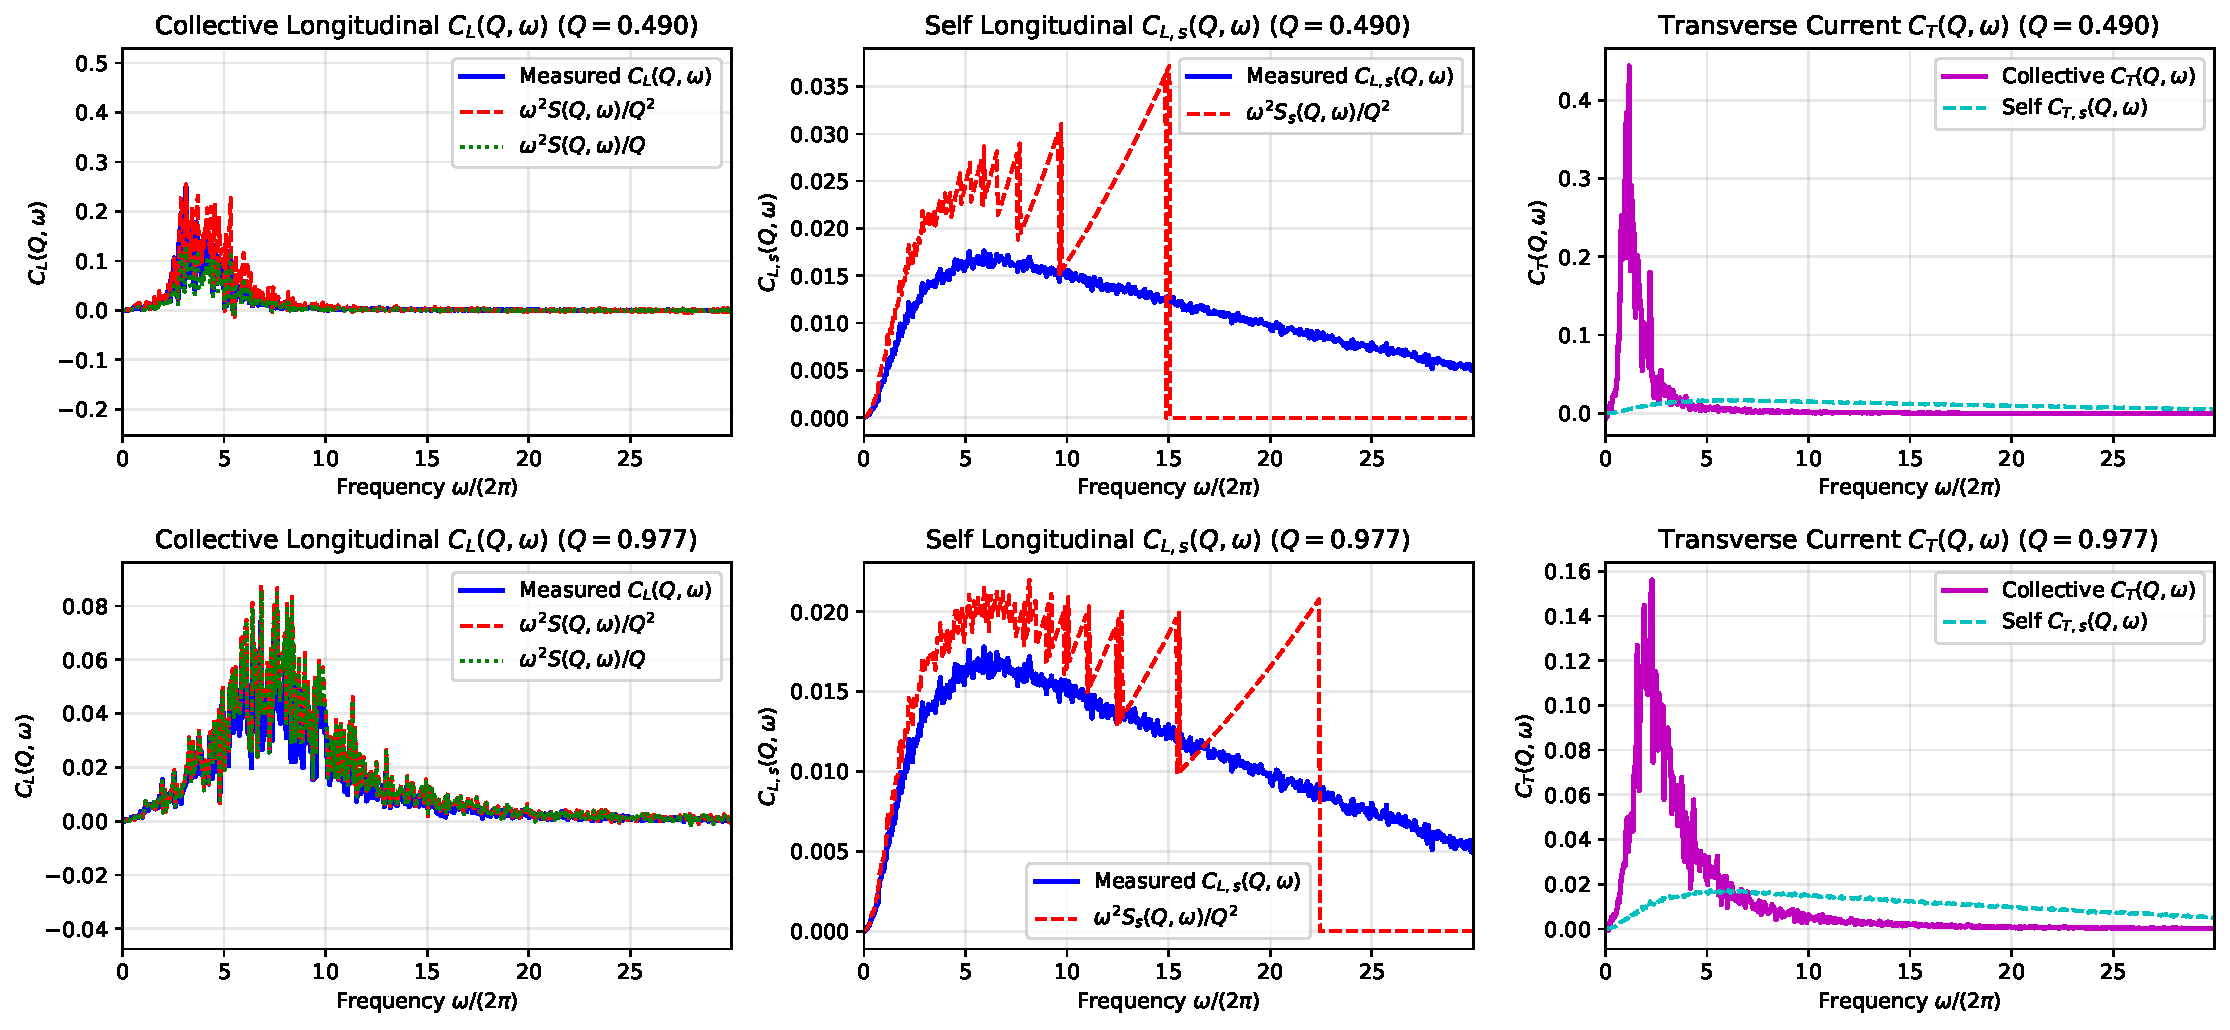
\includegraphics[width=0.95\textwidth]{clqw_spectrum_check.pdf}
\caption{Comparison of collective $C_L(Q,\omega)$ and self $C_{L,s}(Q,\omega)$ longitudinal current spectra for $Q=0.490$ and $Q=0.977$. Prominent Brillouin acoustic peaks indicate collective sound mode propagation.}
\label{fig:spectrum}
\end{figure}

\section{Conclusion}
The implementation of $J_L(Q,t)$ and $C_L(Q,\omega)$ provides a direct, numerically robust route for extracting longitudinal sound velocities $c(Q) = \omega_{\text{peak}}(Q)/Q$ in MD simulations, avoiding high-frequency noise amplification inherent in numerical differentiation of $S(Q,\omega)$.

\end{document}
